\section{Casi d'uso}
\subsection{Introduzione}
In questa sezione vengono presentati i casi d'uso individuati durante l'attività di analisi, 
condotta a partire dal capitolato d'appalto e dagli incontri con il proponente. 
Gli attori vengono identificati in base alla gerarchia trovata e 
alle funzionalità potenziali rilevate.

\subsubsection{Codifica dei casi d'uso}
I casi d'uso sono codificati utilizzando la seguente notazione:

\begin{itemize}
    \item \textbf{UC[ID-Principale][ID-Sottocaso]}: Identificativo univoco del caso d'uso, composto da un ID principale che identifica il caso principale e, se necessario, da un ID del sottocaso.
    \item \textbf{Titolo}: Breve descrizione del caso d'uso.
    \item \textbf{Attori}: Elenco degli attori coinvolti nel caso d'uso.
    \item \textbf{Precondizioni}: Condizioni che devono essere vere prima che il caso d'uso possa iniziare.
    \item \textbf{Postcondizioni}: Condizioni che devono essere vere dopo che il caso d'uso è stato completato con successo.
    \item \textbf{Scenario principale}: Descrizione dettagliata del flusso di eventi principale del caso d'uso.
    \item \textbf{Generalizzazioni}: Eventuali casi d'uso generalizzati.
    \item \textbf{Estensioni}: Eventuali casi d'uso estesi.
    \item \textbf{Inclusione}: Eventuali inclusioni.
\end{itemize}
\newpage
\subsection{Casi d'uso}

\subsubsection{U.C.1 Utilizza chat} %%Esempio
\begin{itemize}
    \item \textbf{Attori}: Utente
    \item \textbf{Precondizioni}: Utente che ha effettuato l'accesso nel sistema.
    \item \textbf{Postcondizioni}: Utente ha effettuato una conversazione.
    \item \textbf{Scenario principale}: L'utente vuole ricevere informazioni riguardanti "\textit{food/beverage}" da acquistare per fornire la sua attività e per farlo avvia una conversazione con il bot.
    \item \textbf{Generalizzazioni}: U.C.1.1, U.C.1.2, U.C.1.3
    \item \textbf{Estensioni}: -
    \item \textbf{Inclusione}: -
\end{itemize}
\begin{figure}[h!]
    \centering
    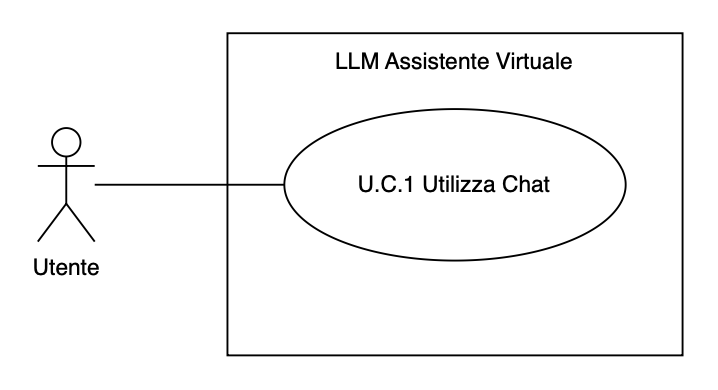
\includegraphics[width=0.5\textwidth]{img/UC1.png}
    \caption{U.C.1 Utilizza Chat}
\end{figure}
\begin{figure}[h!]
    \centering
    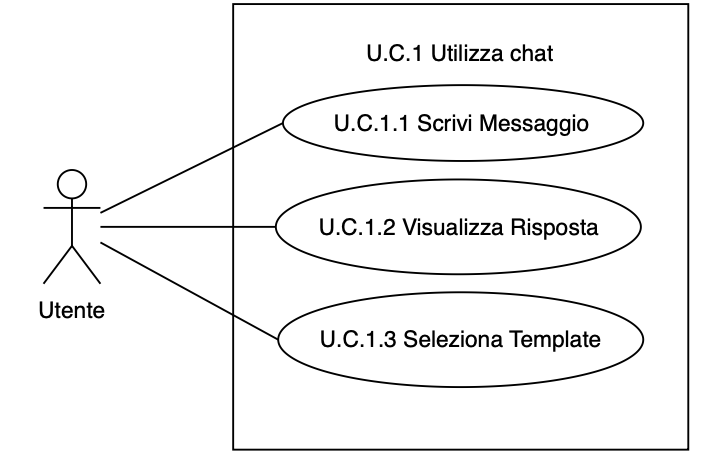
\includegraphics[width=0.5\textwidth]{img/SottocasiUC1.png}
    \caption{Sottocasi di U.C.1}
\end{figure}

\subsubsection{U.C.1.1 Scrivi Messaggio}
\begin{itemize}
    \item \textbf{Attori}: Utente
    \item \textbf{Precondizioni}: Utente che ha effettuato l'accesso nel sistema ed è pronto per effettuare una domanda.
    \item \textbf{Postcondizioni}: L'utente ha inviato un messaggio al bot.
    \item \textbf{Scenario principale}: L’utente vuole domandare al bot delle informazioni riguardo un prodotto o una serie di prodotti.
    \item \textbf{Generalizzazioni}: -
    \item \textbf{Estensioni}: -
    \item \textbf{Inclusione}: -
\end{itemize}
\subsubsection{U.C.1.2 Visualizza Risposta}
\begin{itemize}
    \item \textbf{Attori}: Utente
    \item \textbf{Precondizioni}: Utente che ha effettuato l'accesso ha inviato una domanda al bot.
    \item \textbf{Postcondizioni}: Utente riceve una risposta dal bot coerente alla domanda che ha effettuato.
    \item \textbf{Scenario principale}: L'utente che ha già effettuato la domanda per il bot riceve una risposta coerente sui prodotti.
    \item \textbf{Generalizzazioni}: -
    \item \textbf{Estensioni}: -
    \item \textbf{Inclusione}: -
\end{itemize}
\subsubsection{U.C.1.4 Prodotto non trovato}
\begin{itemize}
    \item \textbf{Attori}: Utente
    \item \textbf{Precondizioni}: Utente che sta conversando con il bot.
    \item \textbf{Postcondizioni}: L'assistente non ha trovato informazioni sul prodotto.
    \item \textbf{Scenario principale}: L’utente richiede domande o informazioni su prodotti non gestiti da noi.
    \item \textbf{Generalizzazioni}: -
    \item \textbf{Estensioni}: -
    \item \textbf{Inclusione}: U.C.13
\end{itemize}
\subsubsection{U.C.13 Invio Richiesta a un Operatore Umano}
\begin{itemize}
    \item \textbf{Attori}: Utente
    \item \textbf{Precondizioni}: L’utente ha ricevuto una risposta non soddisfacente dal sistema basato su LLM.
    \item \textbf{Postcondizioni}: La richiesta dell’utente è stata inviata agli amministratori ed è visibile nella dashboard.
    \item \textbf{Scenario principale}: L’utente seleziona l’opzione per richiedere assistenza a un operatore umano, compila un modulo opzionale con eventuali dettagli e invia la richiesta. Il sistema registra la richiesta e la rende disponibile nella dashboard degli amministratori.
    \item \textbf{Generalizzazioni}: -
    \item \textbf{Estensioni}: -
    \item \textbf{Inclusione}: -
\end{itemize}
\begin{figure}[h!]
    \centering
    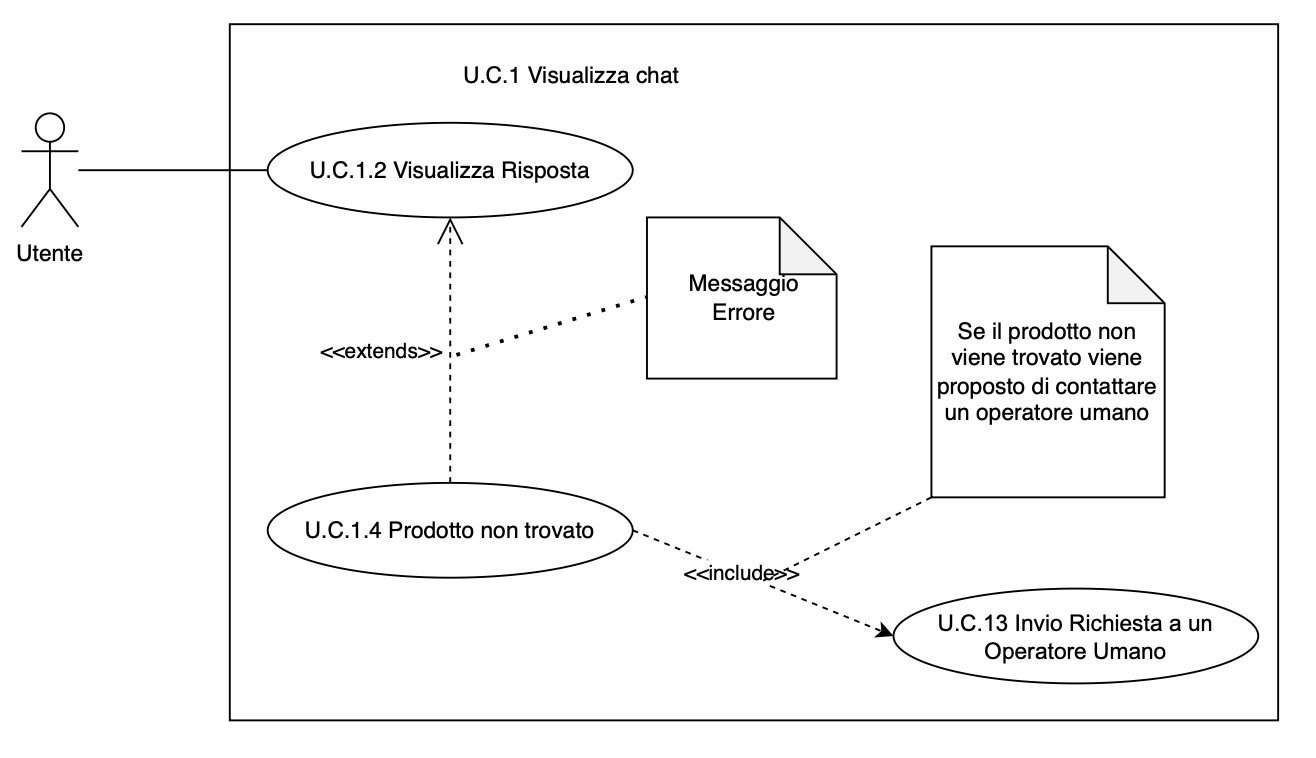
\includegraphics[width=0.8\textwidth]{img/UC1-4.png}
    \caption{U.C.1.4 Prodotto non trovato}
\end{figure}
\subsubsection{U.C.1.3 Seleziona Template}
\begin{itemize}
    \item \textbf{Attori}: Utente
    \item \textbf{Precondizioni}: Utente che ha effettuato l’accesso sta per selezionare una domanda template.
    \item \textbf{Postcondizioni}: Utente ha ricevuto una risposta template (\textit{senza dover chiamare l’LLM}).
    \item \textbf{Scenario principale}: L’utente dentro la chat vuole utilizzare una domanda template tra le consigliate.
    \item \textbf{Generalizzazioni}: -
    \item \textbf{Estensioni}: -
    \item \textbf{Inclusione}: -
\end{itemize}
\subsubsection{U.C.2 Visualizza le conversazioni}
\begin{itemize}
    \item \textbf{Attori}: Utente
    \item \textbf{Precondizioni}: Utente che ha già effettuato l’accesso vuole visualizzare le conversazioni precedentemente salvate.
    \item \textbf{Postcondizioni}: Utente vede una lista di conversazioni salvate.
    \item \textbf{Scenario principale}: L’utente registrato che ha già effettuato una conversazione in passato salvandola vuole visualizzarla di nuovo in un secondo momento.
    \item \textbf{Generalizzazioni}: -
    \item \textbf{Estensioni}: -
    \item \textbf{Inclusione}: U.C.2.1
\end{itemize}
\begin{figure}[h!]
    \centering
    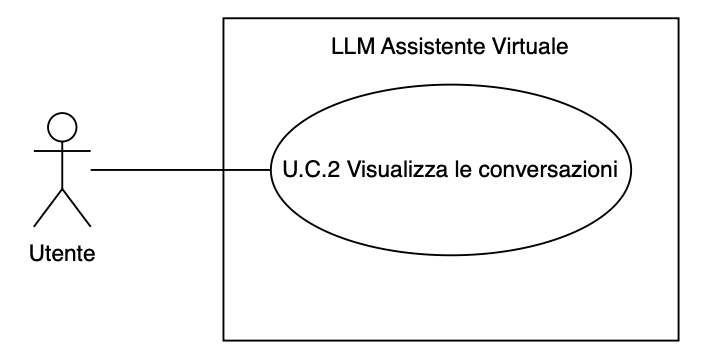
\includegraphics[width=0.5\textwidth]{img/UC2.png}
    \caption{U.C.2 Visualizza le conversazioni}
\end{figure}
\subsubsection{U.C.2.1 Visualizza conversazione singola}
\begin{itemize}
    \item \textbf{Attori}: Utente
    \item \textbf{Precondizioni}: Utente che ha già effettuato l’accesso seleziona una conversazione precedentemente salvata.
    \item \textbf{Postcondizioni}: Utente vede la conversazione precedentemente effettuata.
    \item \textbf{Scenario principale}: L’utente registrato che ha già effettuato una conversazione in passato salvandola vuole visualizzarla di nuovo in un secondo momento.
    \item \textbf{Generalizzazioni}: U.C.2
    \item \textbf{Estensioni}: -
    \item \textbf{Inclusione}: -
\end{itemize}
\begin{figure}[h!]
    \centering
    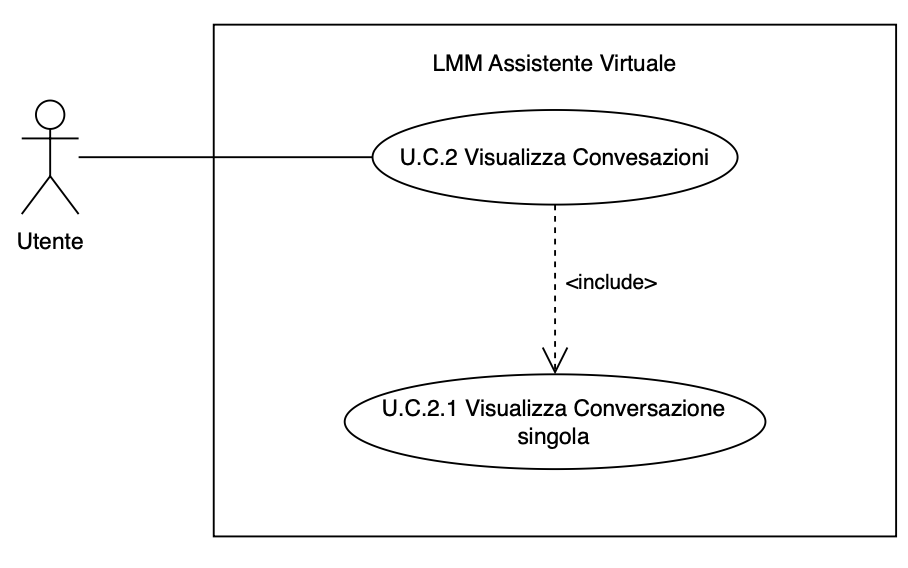
\includegraphics[width=0.6\textwidth]{img/UC2-1.png}
    \caption{U.C.2 Visualizza conversazione singola}
\end{figure}
\subsubsection{U.C.3 Login}
\begin{itemize}
    \item \textbf{Attori}: Utente
    \item \textbf{Precondizioni}: Utente già registrato.
    \item \textbf{Postcondizioni}: Utente ha effettuato l'accesso.
    \item \textbf{Scenario principale}: L'utente già registrato vuole accedere al sistema.
    \item \textbf{Generalizzazioni}: -
    \item \textbf{Estensioni}: -
    \item \textbf{Inclusione}: -
\end{itemize}
\begin{figure}[h!]
    \centering
    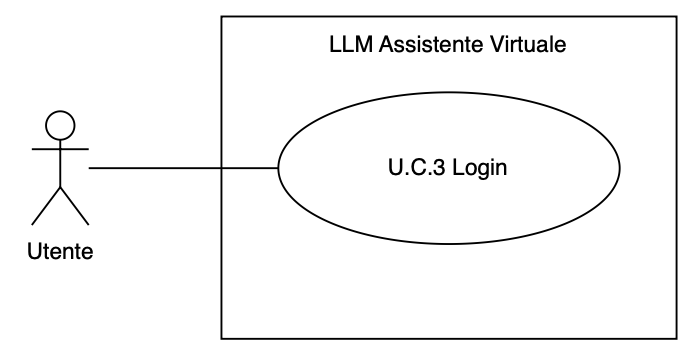
\includegraphics[width=0.5\textwidth]{img/UC3.png}
    \caption{U.C.3 Login}
\end{figure}
\begin{figure}[h!]
    \centering
    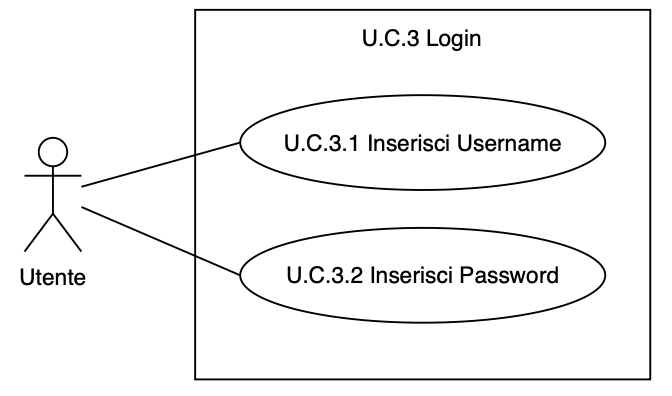
\includegraphics[width=0.5\textwidth]{img/UC3p1.png}
    \caption{Sottocasi di U.C.3}
\end{figure}
\subsubsection{U.C.3.1 Inserisci Username}
\begin{itemize}
    \item \textbf{Attori}: Utente
    \item \textbf{Precondizioni}: Utente già registrato.
    \item \textbf{Postcondizioni}: Utente ha inserito un Username.
    \item \textbf{Scenario principale}: L'utente già registrato vuole accedere al sistema.
    \item \textbf{Generalizzazioni}: -
    \item \textbf{Estensioni}: U.C.3.4, U.C.3.5
    \item \textbf{Inclusione}: -
\end{itemize}
\subsubsection{U.C.3.4 Username errato}
\begin{itemize}
    \item \textbf{Attori}: Utente
    \item \textbf{Precondizioni}: Utente già registrato.
    \item \textbf{Postcondizioni}: Utente ha inserito un username errato e gli viene impedito di accedere al sistema.
    \item \textbf{Scenario principale}: L’utente ha provato ad accedere al sistema utilizzando un username errato e viene visualizzato un messaggio di errore generico.
    \item \textbf{Generalizzazioni}: -
    \item \textbf{Estensioni}: -
    \item \textbf{Inclusione}: -
\end{itemize}
\begin{figure}[h!]
    \centering
    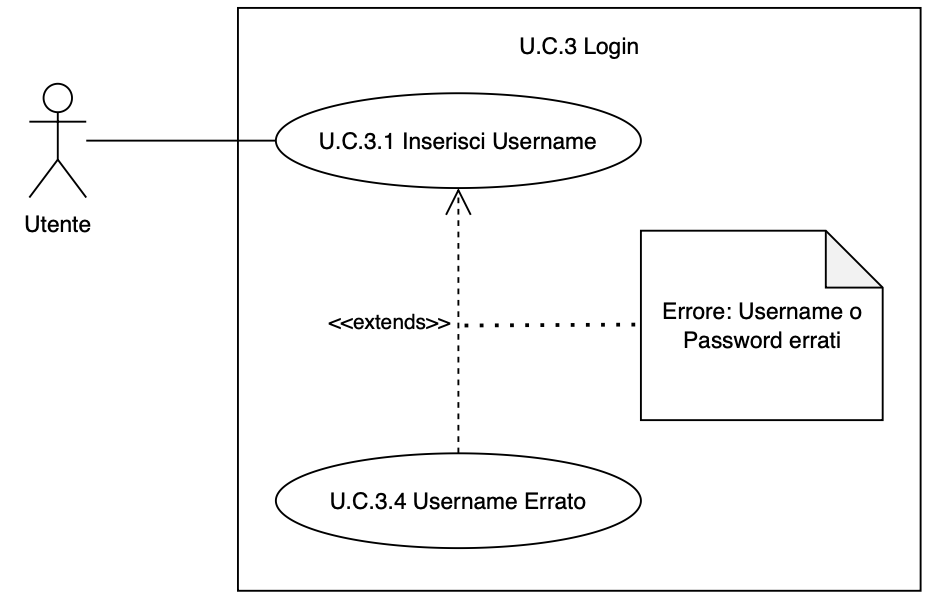
\includegraphics[width=0.6\textwidth]{img/UC3-4.png}
    \caption{U.C.3.4 Username errato}
\end{figure}
\subsubsection{U.C.3.2 Inserisci Password}
\begin{itemize}
    \item \textbf{Attori}: Utente
    \item \textbf{Precondizioni}: Utente già registrato.
    \item \textbf{Postcondizioni}: Utente ha inserito una Password.
    \item \textbf{Scenario principale}: L'utente già registrato vuole accedere al sistema.
    \item \textbf{Generalizzazioni}: -
    \item \textbf{Estensioni}: U.C.3.3, U.C.3.5
    \item \textbf{Inclusione}: -
\end{itemize}
\subsubsection{U.C.3.3 Password Errata}
\begin{itemize}
    \item \textbf{Attori}: Utente
    \item \textbf{Precondizioni}: Utente già registrato
    \item \textbf{Postcondizioni}: Utente ha inserito una password errata e gli viene impedito di accedere al sistema
    \item \textbf{Scenario principale}: L'utente ha provato ad accedere al sistema utilizzando una password errata e viene visualizzato un messaggio di errore generico
    \item \textbf{Generalizzazioni}: -
    \item \textbf{Estensioni}: -
    \item \textbf{Inclusione}: -
\end{itemize}
\begin{figure}[h!]
    \centering
    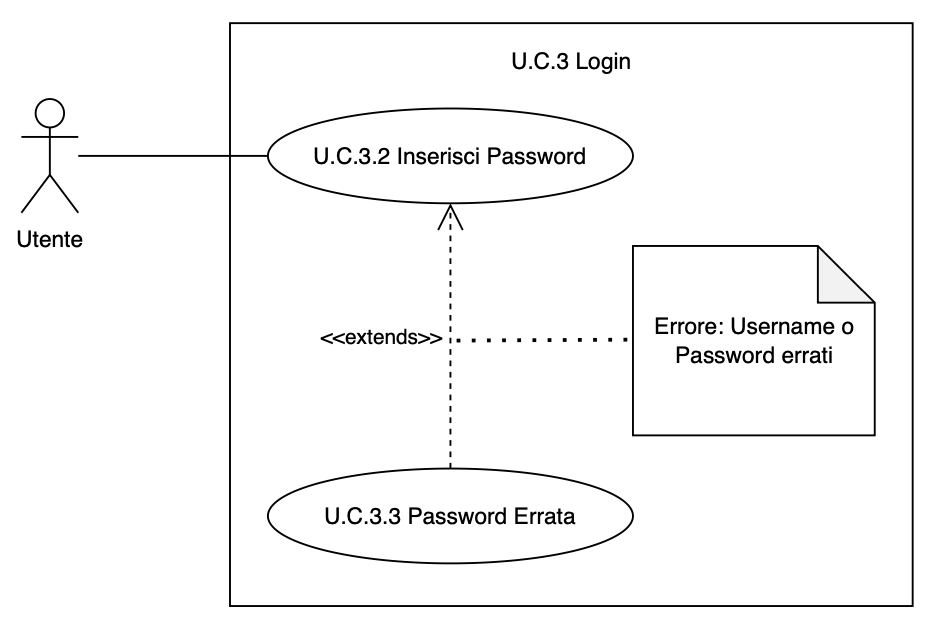
\includegraphics[width=0.7\textwidth]{img/UC3-3.png}
    \caption{U.C.3.3 Password errata}
\end{figure}
\subsubsection{U.C.3.5 Caratteri non validi}
\begin{itemize}
    \item \textbf{Attori}: Utente
    \item \textbf{Precondizioni}: Utente già registrato
    \item \textbf{Postcondizioni}: Utente ha inserito caratteri particolari e gli viene impedito di accedere al sistema
    \item \textbf{Scenario principale}: L’utente ha provato ad entrare nel sistema cercando di rompere o rubare informazioni e gli viene impedito di entrare nel sistema
    \item \textbf{Generalizzazioni}: -
    \item \textbf{Estensioni}: -
    \item \textbf{Inclusione}: -
\end{itemize}
\begin{figure}[h!]
    \centering
    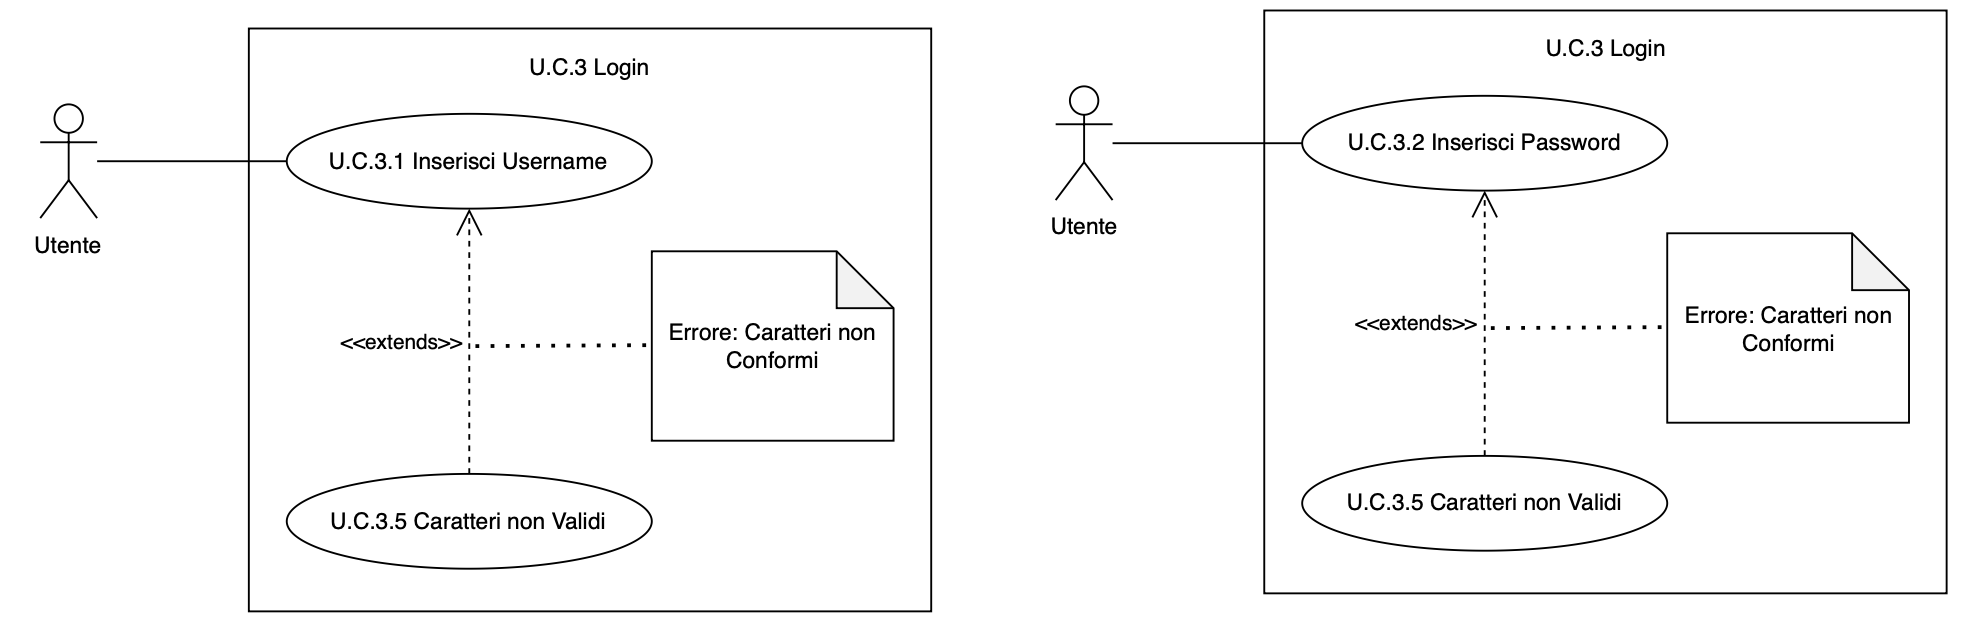
\includegraphics[width=\textwidth]{img/UC3-5.png}
    \caption{U.C.3.5 Caratteri non validi}
\end{figure}
\subsubsection{U.C.4 Sign Up}
\begin{itemize}
    \item \textbf{Attori}: Utente
    \item \textbf{Precondizioni}: Utente non registrato
    \item \textbf{Postcondizioni}: L'utente viene registrato
    \item \textbf{Scenario principale}: L’utente non registrato vuole usufruire del servizio registrandosi
    \item \textbf{Generalizzazioni}: -
    \item \textbf{Estensioni}: -
    \item \textbf{Inclusione}: -
\end{itemize}
\begin{figure}[h!]
    \centering
    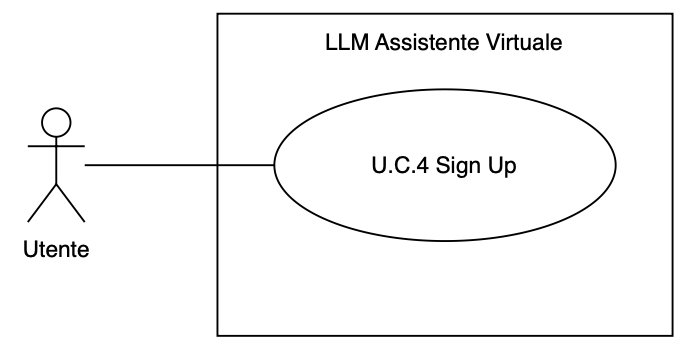
\includegraphics[width=0.5\textwidth]{img/UC4.png}
    \caption{U.C.4 Sign Up}
\end{figure}
\begin{figure}[h!]
    \centering
    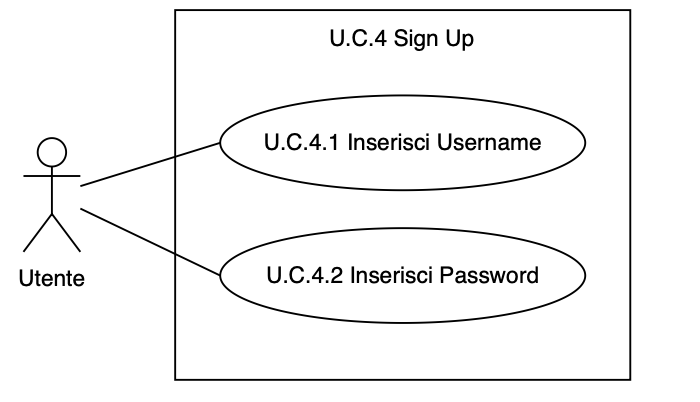
\includegraphics[width=0.5\textwidth]{img/UC4p1.png}
    \caption{U.C.4 Sottocasi di U.C.4}
\end{figure}
\newpage
\subsubsection{U.C.4.4 Username troppo lungo}
\begin{itemize}
    \item \textbf{Attori}: Utente
    \item \textbf{Precondizioni}: Utente non registrato inserisce un username
    \item \textbf{Postcondizioni}: All'utente non viene permessa la registrazione
    \item \textbf{Scenario principale}: L’utente non registrato vuole registrarsi nel sistema ma gli viene impedito a causa di un username troppo lungo
    \item \textbf{Generalizzazioni}: -
    \item \textbf{Estensioni}: -
    \item \textbf{Inclusione}: -
\end{itemize}
\begin{figure}[h!]
    \centering
    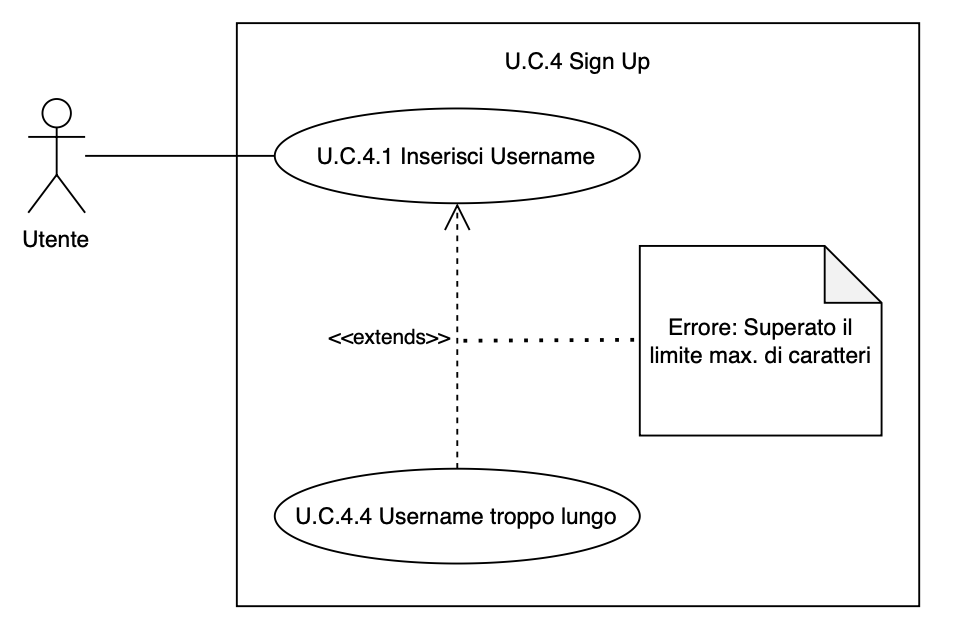
\includegraphics[width=0.5\textwidth]{img/UC4-4.png}
    \caption{U.C.4.4 Username troppo lungo}
\end{figure}
\newpage
\subsubsection{U.C.4.6 Username già presente}
\begin{itemize}
    \item \textbf{Attori}: Utente
    \item \textbf{Precondizioni}: Utente non registrato inserisce un username
    \item \textbf{Postcondizioni}: All'utente non viene permessa la registrazione
    \item \textbf{Scenario principale}: L’utente non registrato vuole registrarsi nel sistema ma gli viene impedito a causa di uno stesso username già presente nel sistema
    \item \textbf{Generalizzazioni}: -
    \item \textbf{Estensioni}: -
    \item \textbf{Inclusione}: -
\end{itemize}
\begin{figure}[h!]
    \centering
    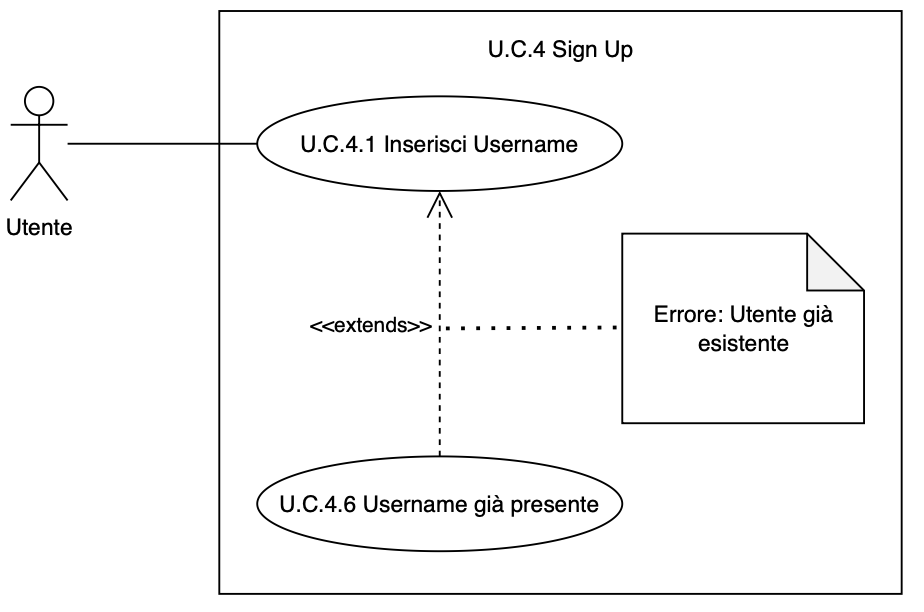
\includegraphics[width=0.5\textwidth]{img/UC4-6.png}
    \caption{U.C.4.6 Username già presente}
\end{figure}
\subsubsection{U.C.4.2 Inserisci Password}
\begin{itemize}
    \item \textbf{Attori}: Utente
    \item \textbf{Precondizioni}: Utente non registrato inserisce una password
    \item \textbf{Postcondizioni}: Utente dichiara al sistema la sua parola di accesso
    \item \textbf{Scenario principale}: L’utente non registrato vuole registrarsi nel sistema
    \item \textbf{Generalizzazioni}: -
    \item \textbf{Estensioni}: U.C.4.3, U.C.4.5
    \item \textbf{Inclusione}: -
\end{itemize}
\subsubsection{U.C.4.5 Password troppo lunga}
\begin{itemize}
    \item \textbf{Attori}: Utente
    \item \textbf{Precondizioni}: Utente non registrato inserisce una password
    \item \textbf{Postcondizioni}: All'utente non viene permessa la registrazione
    \item \textbf{Scenario principale}: L’utente non registrato vuole registrarsi nel sistema ma gli viene impedito a causa di una password troppo lunga
    \item \textbf{Generalizzazioni}: -
    \item \textbf{Estensioni}: -
    \item \textbf{Inclusione}: -
\end{itemize}
\begin{figure}[h!]
    \centering
    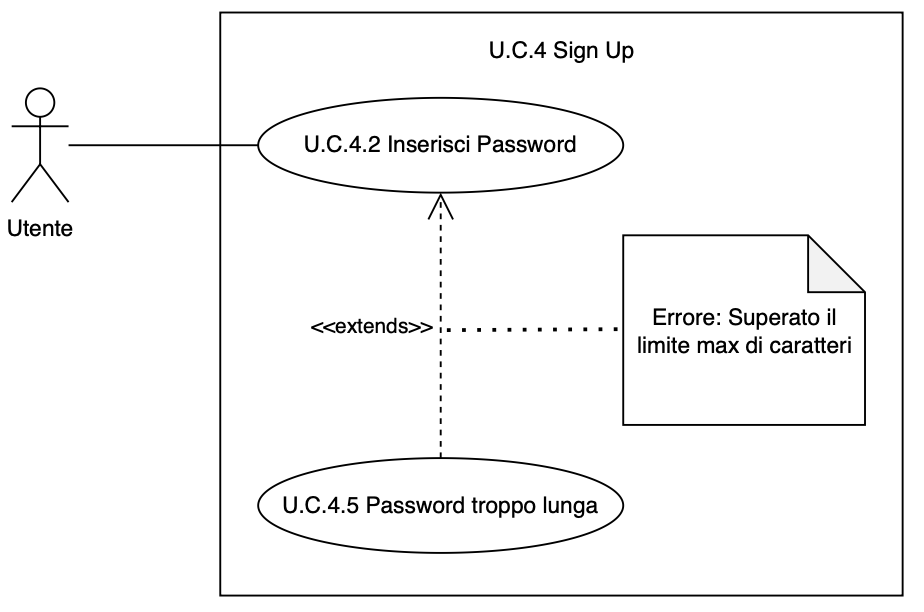
\includegraphics[width=0.5\textwidth]{img/UC4-5.png}
    \caption{U.C.4.5 Password troppo lunga}
\end{figure}
\subsubsection{U.C.4.3 Caratteri non validi}
\begin{itemize}
    \item \textbf{Attori}: Utente
    \item \textbf{Precondizioni}: Utente non registrato inserisce una password
    \item \textbf{Postcondizioni}: All'utente non viene permessa la registrazione
    \item \textbf{Scenario principale}: L'utente ha provato a rompere il sistema e gli viene impedito di accedere a questo
    \item \textbf{Generalizzazioni}: -
    \item \textbf{Estensioni}: -
    \item \textbf{Inclusione}: -
\end{itemize}
\begin{figure}[h!]
    \centering
    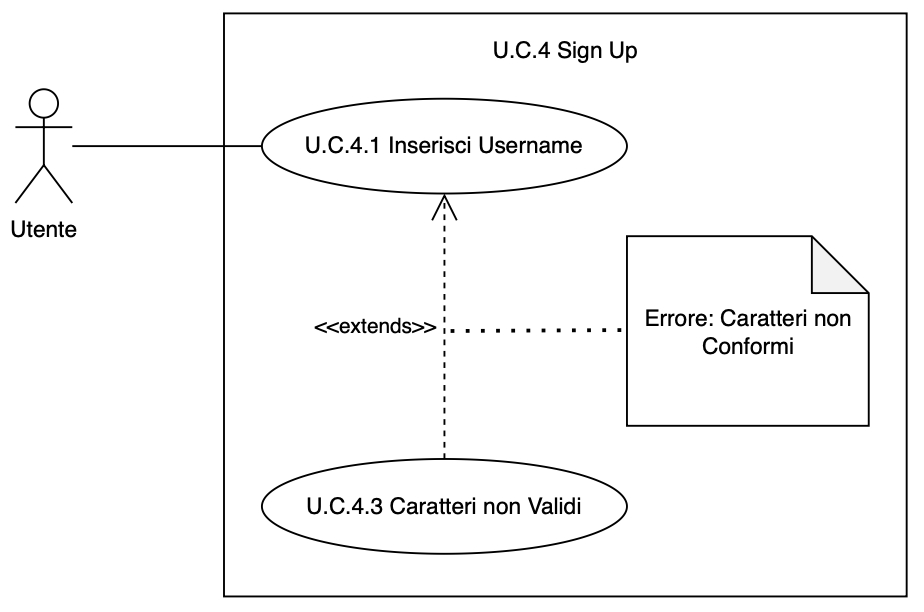
\includegraphics[width=0.5\textwidth]{img/UC4-3.png}
    \caption{U.C.4.3 estensione di U.C.4.1}
\end{figure}
\begin{figure}[h!]
    \centering
    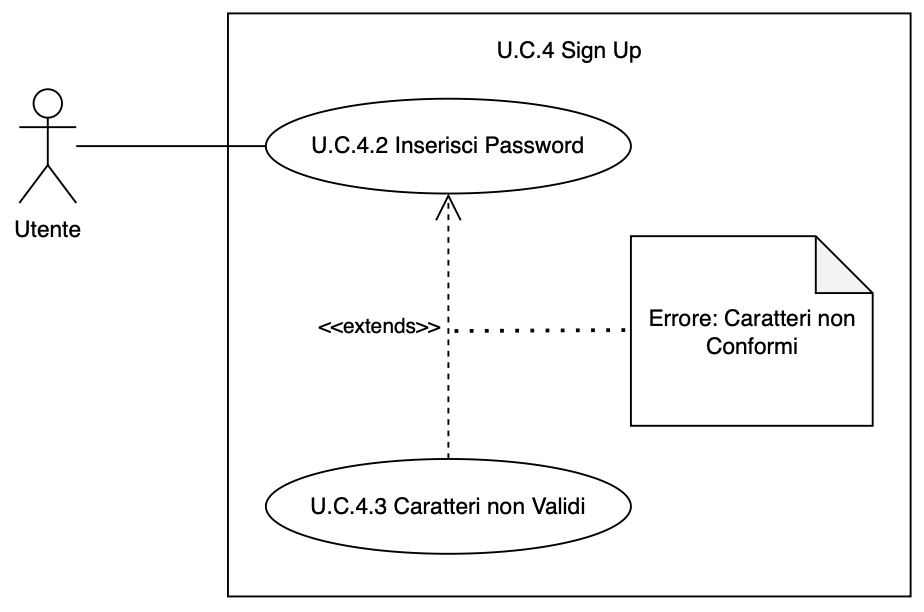
\includegraphics[width=0.5\textwidth]{img/UC4-3-2.png}
    \caption{U.C.4.3 estensione di U.C.4.2}
\end{figure}
\subsubsection{U.C.5 Salva Chat}
\begin{itemize}
    \item \textbf{Attori}: Utente
    \item \textbf{Precondizioni}: Utente che ha effettuato l'accesso ed è in conversazione con il bot.
    \item \textbf{Postcondizioni}: L'utente ha salvato la conversazione.
    \item \textbf{Scenario principale}: L'utente, dopo aver effettuato le sue domande, vuole salvarle per visualizzarle in un secondo momento.
    \item \textbf{Generalizzazioni}: -
    \item \textbf{Estensioni}: U.C.5.1
    \item \textbf{Inclusione}: -
\end{itemize}
\begin{figure}[h!]
    \centering
    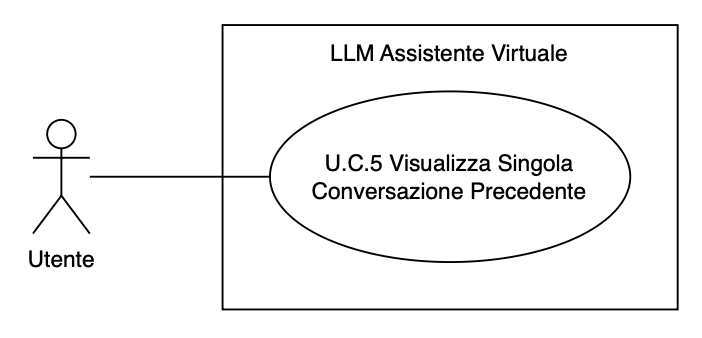
\includegraphics[width=0.5\textwidth]{img/UC5.png}
    \caption{U.C.5 Salva Chat}
\end{figure}
\subsubsection{U.C.5.1 Memoria Piena}
\begin{itemize}
    \item \textbf{Attori}: Utente
    \item \textbf{Precondizioni}: Utente che ha effettuato l'accesso vuole salvare la conversazione.
    \item \textbf{Postcondizioni}: L'utente non ha potuto conservare la conversazione.
    \item \textbf{Scenario principale}: L’utente, dopo aver effettuato le sue domande, vuole salvarle per visualizzarle in un secondo momento, tuttavia questo non è possibile dato che la memoria dedicata alle chat del suo account è terminata \textit{(dovrà cancellarne alcune per liberarla)}.
    \item \textbf{Generalizzazioni}: -
    \item \textbf{Estensioni}: -
    \item \textbf{Inclusione}: -
\end{itemize}
\begin{figure}[h!]
    \centering
    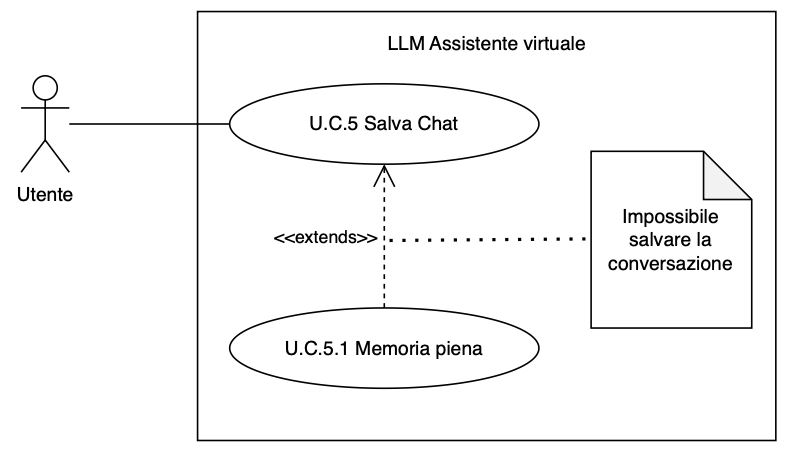
\includegraphics[width=0.5\textwidth]{img/UC5-1.png}
    \caption{U.C.5.1 Memoria Piena}
\end{figure}
\subsubsection{U.C.10 Elimina Chat}
\begin{itemize}
    \item \textbf{Attori}: Utente
    \item \textbf{Precondizioni}: Utente che ha effettuato l'accesso ed ha effettuato una conversazione.
    \item \textbf{Postcondizioni}: La conversazione scelta è stata eliminata.
    \item \textbf{Scenario principale}: L'utente vuole eliminare una conversazione.
    \item \textbf{Generalizzazioni}: -
    \item \textbf{Estensioni}: -
    \item \textbf{Inclusione}: -
\end{itemize}
\begin{figure}[h!]
    \centering
    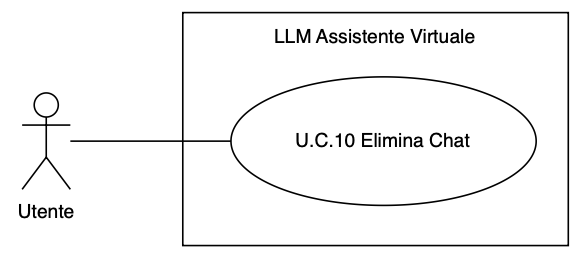
\includegraphics[width=0.5\textwidth]{img/UC10.png}
    \caption{U.C.10 Elimina chat}
\end{figure}
\newpage
\subsubsection{U.C.11 Riprendi Conversazione}
\begin{itemize}
    \item \textbf{Attori}: Utente
    \item \textbf{Precondizioni}: L’utente ha effettuato l’accesso al sistema ed effettuato una conversazione.
    \item \textbf{Postcondizioni}: L’utente riprende la conversazione con l’assistente virtuale.
    \item \textbf{Scenario principale}: L’utente ha per qualche motivo dovuto interrompere la conversazione e la riprende successivamente in un secondo momento.
    \item \textbf{Generalizzazioni}: -
    \item \textbf{Estensioni}: -
    \item \textbf{Inclusione}: -
\end{itemize}
\begin{figure}[h!]
    \centering
    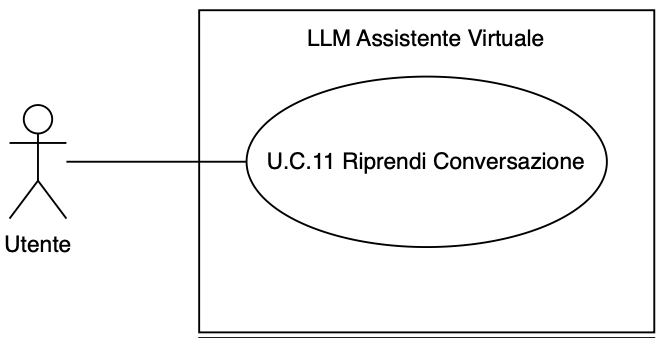
\includegraphics[width=0.5\textwidth]{img/UC11.png}
    \caption{U.C.11 Riprendi Conversazione}
\end{figure}
\subsubsection{U.C.6 Feedback Chat}
\begin{itemize}
    \item \textbf{Attori}: Utente
    \item \textbf{Precondizioni}: Utente che ha effettuato l'accesso e concluso una conversazione.
    \item \textbf{Postcondizioni}: L'utente ha dato un Feedback sulla conversazione.
    \item \textbf{Scenario principale}: L'utente, dopo aver effettuato una conversazione, vuole successivamente dare un Feedback sulla qualità (\textit{positivo-negativo}) della risposta.
    \item \textbf{Generalizzazioni}: -
    \item \textbf{Estensioni}: -
    \item \textbf{Inclusione}: U.C.13
\end{itemize}
\begin{figure}[h!]
    \centering
    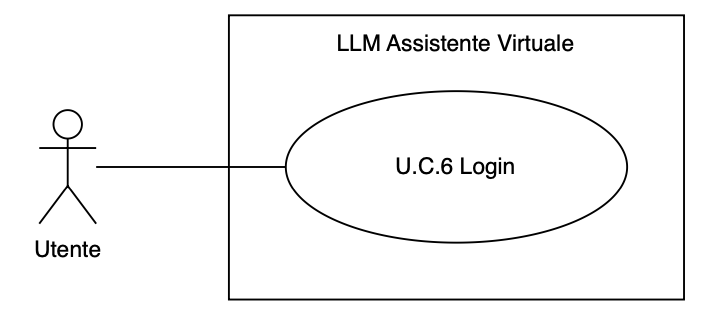
\includegraphics[width=0.8\textwidth]{img/UC6.png}
    \caption{U.C.6 Feedback chat}
\end{figure}
\subsubsection{U.C.7 Configurazione Template Domande e Risposte}
\begin{itemize}
    \item \textbf{Attori}: Admin
    \item \textbf{Precondizioni}: L’amministratore ha effettuato l’accesso alla piattaforma di gestione.
    \item \textbf{Postcondizioni}: Il sistema salva i nuovi template o aggiorna quelli esistenti.
    \item \textbf{Scenario principale}: L’amministratore accede alla sezione di configurazione, crea o modifica template di domande e risposte, e salva i cambiamenti.
    \item \textbf{Generalizzazioni}: -
    \item \textbf{Estensioni}: -
    \item \textbf{Inclusione}: -
\end{itemize}
\begin{figure}[h!]
    \centering
    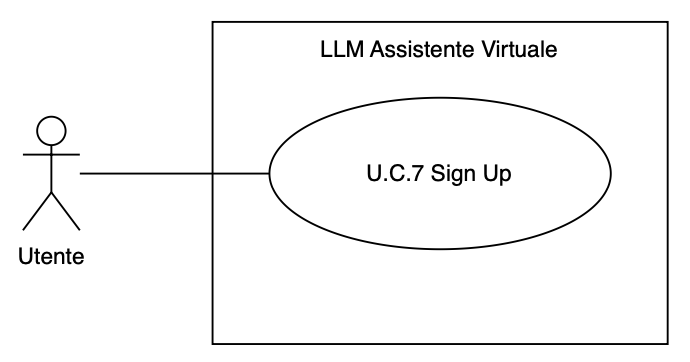
\includegraphics[width=0.5\textwidth]{img/UC7.png}
    \caption{U.C.7 Configurazione Template Domande e Risposte}
\end{figure}
\begin{figure}[h!]
    \centering
    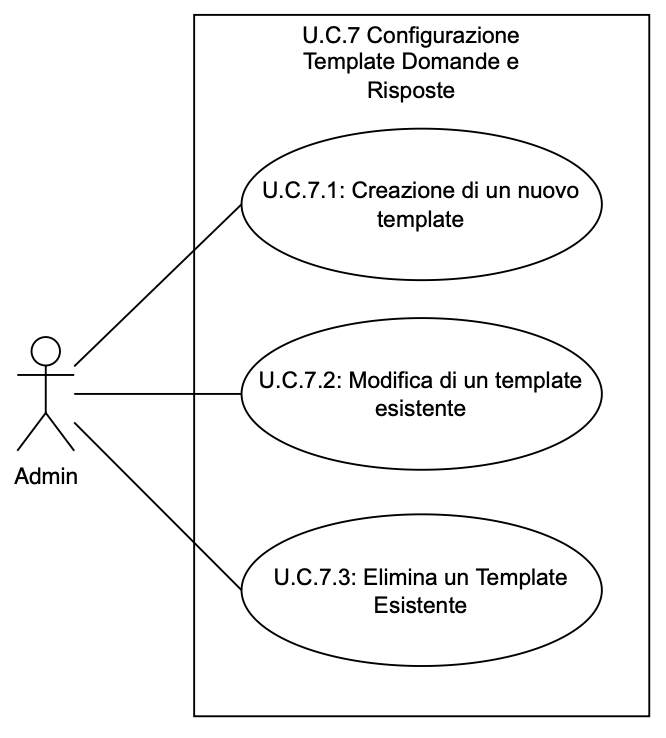
\includegraphics[width=0.5\textwidth]{img/UC7p1.png}
    \caption{Sottocasi di U.C.7}
\end{figure}
\newpage
\subsubsection{U.C.7.1 Creazione di un nuovo template}
\begin{itemize}
    \item \textbf{Attori}: Admin
    \item \textbf{Precondizioni}: L’amministratore ha effettuato l’accesso e selezionato la categoria di interesse.
    \item \textbf{Postcondizioni}: Un nuovo template è stato aggiunto con una domanda e una risposta associata.
    \item \textbf{Scenario principale}: L’amministratore compila i campi richiesti per la nuova domanda e la salva.
    \item \textbf{Generalizzazioni}: -
    \item \textbf{Estensioni}: -
    \item \textbf{Inclusione}: -
\end{itemize}
%%%%%%%%%%%%%%%%%%%%%%%%%%%%%%%%%%%%%%%%%%%%%%%%%AGGIUNGERE IMMAGINI E UC7.4 DOPO CONFERMA
%%%%%%%%%%%%%%%%%%%%%%%%%%%%%%%%%%%%%%%%%%%%%%%%%
\subsubsection{U.C.7.2 Modifica di un template esistente}
\begin{itemize}
    \item \textbf{Attori}: Admin
    \item \textbf{Precondizioni}: L’amministratore ha effettuato l’accesso e selezionato un template esistente.
    \item \textbf{Postcondizioni}: Il template selezionato è stato aggiornato.
    \item \textbf{Scenario principale}: L’amministratore modifica i dettagli di un template già esistente e salva le modifiche.
    \item \textbf{Generalizzazioni}: -
    \item \textbf{Estensioni}: -
    \item \textbf{Inclusione}: -
\end{itemize}
\subsubsection{U.C.7.3 Elimina un template esistente}
\begin{itemize}
    \item \textbf{Attori}: Admin
    \item \textbf{Precondizioni}: L’amministratore ha effettuato l’accesso e selezionato un template esistente.
    \item \textbf{Postcondizioni}: Il template selezionato è stato eliminato.
    \item \textbf{Scenario principale}: L'amministratore elimina il template.
    \item \textbf{Generalizzazioni}: -
    \item \textbf{Estensioni}: -
    \item \textbf{Inclusione}: -
\end{itemize}
%%%%%%%%%%%AGGIUNGERE QUI UC7.4 IN CASO%%%%%%%%%%%%
%%%%%%%%%%%%%%%%%%%%%%%%%%%%%%%%%%%%%%%%%%%%%%%%%%%%%%%%%%%%%%%%%%%%%%%%%%%%%%%%%%%%%%%%%%%%
\subsubsection{U.C.8 Monitoraggio delle Prestazioni del Sistema}
\begin{itemize}
    \item \textbf{Attori}: Admin
    \item \textbf{Precondizioni}: L’amministratore ha effettuato l’accesso alla dashboard di monitoraggio.
    \item \textbf{Postcondizioni}: L’amministratore ha consultato le metriche o identificato anomalie nel sistema.
    \item \textbf{Scenario principale}: L’amministratore visualizza il tempo medio di risposta, il numero di richieste e altre statistiche.
    \item \textbf{Generalizzazioni}: -
    \item \textbf{Estensioni}: -
    \item \textbf{Inclusione}: -
\end{itemize}
\begin{figure}[h!]
    \centering
    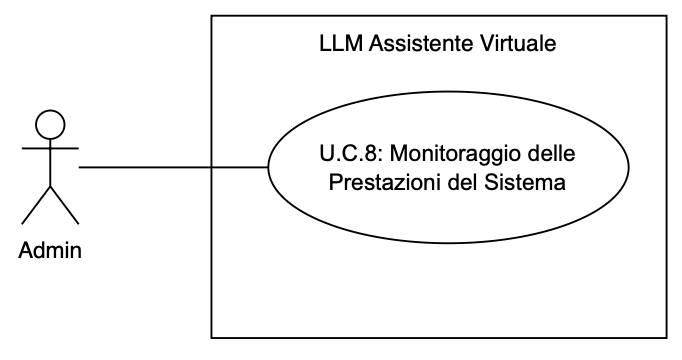
\includegraphics[width=0.5\textwidth]{img/UC8.png}
    \caption{U.C.8 Monitoraggio delle Prestazioni del Sistema}
\end{figure}
\begin{figure}[h!]
    \centering
    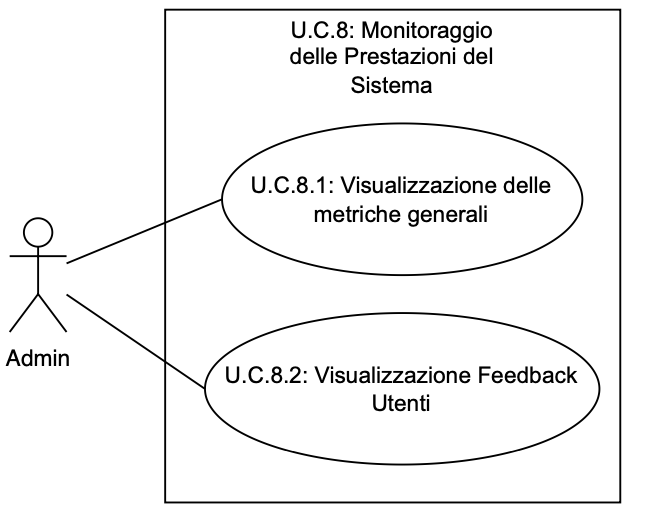
\includegraphics[width=0.5\textwidth]{img/UC8p1.png}
    \caption{Sottocasi di U.C.8}
\end{figure}
\subsubsection{U.C.8.1 Visualizzazione delle metriche generali}
\begin{itemize}
    \item \textbf{Attori}: Admin
    \item \textbf{Precondizioni}: L’amministratore ha effettuato l’accesso alla dashboard.
    \item \textbf{Postcondizioni}: Le metriche principali sono state visualizzate.
    \item \textbf{Scenario principale}: L’amministratore consulta le statistiche generali del sistema per un periodo di tempo specifico.
    \item \textbf{Generalizzazioni}: -
    \item \textbf{Estensioni}: -
    \item \textbf{Inclusione}: -
\end{itemize}
\subsubsection{U.C.8.2 Visualizzazione Feedback Utenti}
\begin{itemize}
    \item \textbf{Attori}: Admin
    \item \textbf{Precondizioni}: L’amministratore ha effettuato l’accesso alla dashboard e ha consultato le metriche.
    \item \textbf{Postcondizioni}: L’amministratore visualizza i feedback degli utenti.
    \item \textbf{Scenario principale}: L’amministratore visualizza i feedback sulle risposte dell’LLM degli utenti.
    \item \textbf{Generalizzazioni}: -
    \item \textbf{Estensioni}: -
    \item \textbf{Inclusione}: -
\end{itemize}
\subsubsection{U.C.9 Gestione Database Relazionale Dati Aziendali}
\begin{itemize}
    \item \textbf{Attori}: Admin
    \item \textbf{Precondizioni}: L’amministratore ha effettuato l’accesso al sistema e ha caricato un file di dati.
    \item \textbf{Postcondizioni}: Il Database è stato aggiornato con i nuovi dati.
    \item \textbf{Scenario principale}: L’amministratore importa nuovi dati sui prodotti, il sistema li valida e li salva.
    \item \textbf{Generalizzazioni}: -
    \item \textbf{Estensioni}: -
    \item \textbf{Inclusione}: -
\end{itemize}
\begin{figure}[h!]
    \centering
    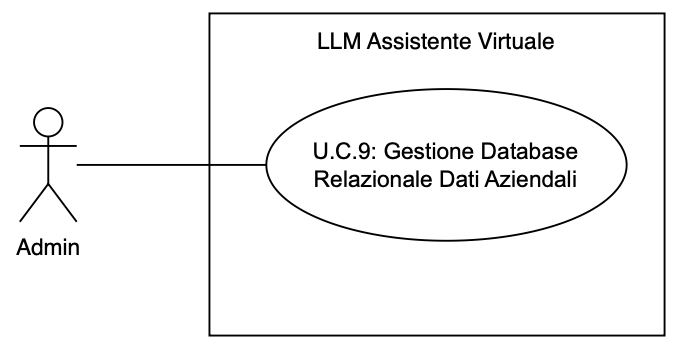
\includegraphics[width=0.5\textwidth]{img/UC9.png}
    \caption{U.C.9 Gestione Database Relazionale Dati Aziendali}
\end{figure}
\begin{figure}[h!]
    \centering
    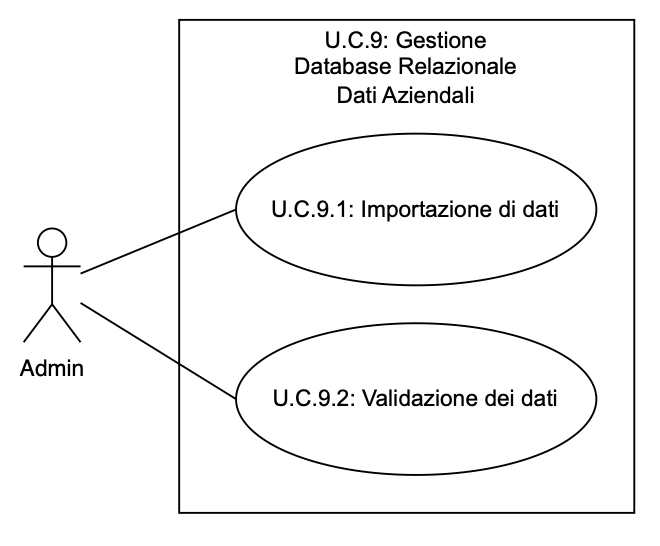
\includegraphics[width=0.5\textwidth]{img/UC9p1.png}
    \caption{Sottocasi di U.C.9}
\end{figure}
\subsubsection{U.C.9.1 Importazione di Dati}
\begin{itemize}
    \item \textbf{Attori}: Admin
    \item \textbf{Precondizioni}: L’amministratore ha effettuato l’accesso e selezionato un file da importare.
    \item \textbf{Postcondizioni}: I dati sono stati caricati per la validazione.
    \item \textbf{Scenario principale}: L’amministratore carica il file con i nuovi dati sul sistema.
    \item \textbf{Generalizzazioni}: -
    \item \textbf{Estensioni}: -
    \item \textbf{Inclusione}: -
\end{itemize}
\subsubsection{U.C.9.2 Validazione di Dati}
\begin{itemize}
    \item \textbf{Attori}: Sistema
    \item \textbf{Precondizioni}: Un file di dati è stato caricato correttamente.
    \item \textbf{Postcondizioni}: Il sistema ha validato o respinto il file.
    \item \textbf{Scenario principale}: Il sistema controlla il formato e la coerenza dei dati.
    \item \textbf{Generalizzazioni}: -
    \item \textbf{Estensioni}: -
    \item \textbf{Inclusione}: -
\end{itemize}
\subsubsection{U.C.12 Gestione richieste Contatti}
\begin{itemize}
    \item \textbf{Attori}: Admin
    \item \textbf{Precondizioni}: L’amministratore ha effettuato l’accesso al sistema e in seguito alla dashboard per la gestione delle richieste di contatto.
    \item \textbf{Postcondizioni}: L’amministratore ha gestito le richieste di contatto degli utenti.
    \item \textbf{Scenario principale}: L’amministratore accede alla dashboard delle richieste di contatto e interagisce con le richieste per effettuare “servizio clienti”. Dopo aver selezionato una richiesta, risponde tramite email e aggiorna lo stato come "gestita".
    \item \textbf{Generalizzazioni}: -
    \item \textbf{Estensioni}: -
    \item \textbf{Inclusione}: -
\end{itemize}
\begin{figure}[h!]
    \centering
    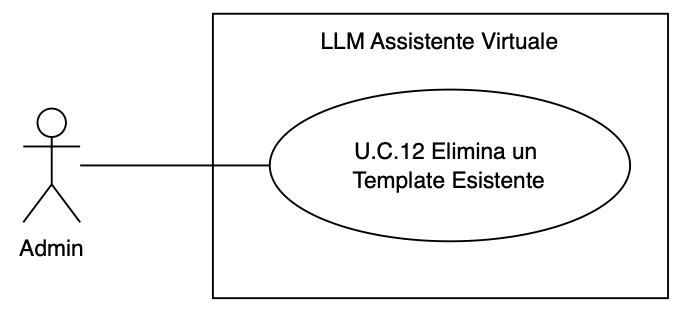
\includegraphics[width=0.5\textwidth]{img/UC12.png}
    \caption{U.C.12 Gestione richieste Contatti}
\end{figure}
\subsubsection{U.C.12.1 Risposta alla Richiesta dall'amministratore}
\begin{itemize}
    \item \textbf{Attori}: Admin
    \item \textbf{Precondizioni}: L’amministratore ha effettuato l’accesso al sistema e in seguito alla dashboard per la gestione delle richieste di contatto. È presente almeno una richiesta inviata da un utente.
    \item \textbf{Postcondizioni}: L’amministratore ha risposto alla richiesta tramite email. La richiesta è stata aggiornata come "gestita".
    \item \textbf{Scenario principale}: L’amministratore accede alla dashboard, seleziona una richiesta da gestire e ne visualizza i dettagli. Compone una risposta e la invia tramite il sistema. Infine, aggiorna lo stato della richiesta come "gestita".
    \item \textbf{Generalizzazioni}: -
    \item \textbf{Estensioni}: -
    \item \textbf{Inclusione}: -
\end{itemize}
\begin{figure}[h!]
    \centering
    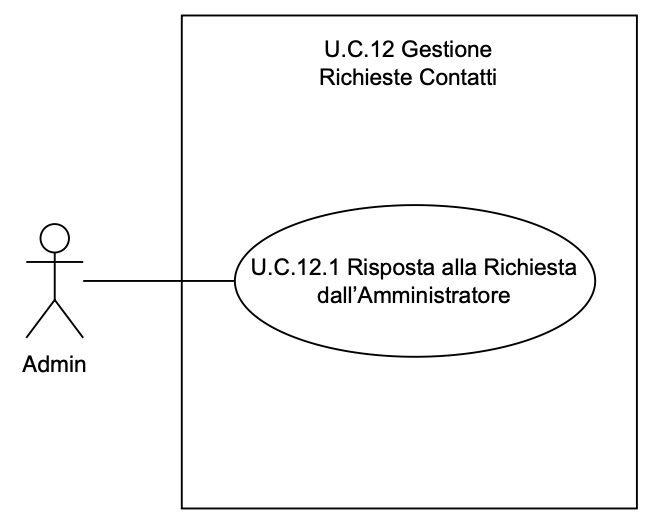
\includegraphics[width=0.5\textwidth]{img/UC12-1.png}
    \caption{U.C.12.1 Risposta alla Richiesta dall'amministratore}
\end{figure}
\newpage
